\documentclass[11pt]{article}
\usepackage{todonotes}
\usepackage{fullpage}
\usepackage{amsmath}
\usepackage{setspace}
\usepackage{listings}
\usepackage{verbatim}
\usepackage{algpseudocode}
\usepackage{algorithm}
\usepackage{caption}
\algblockdefx[IF]{If}{EndIf}[1]{\algorithmicif\ #1}{\algorithmicend}
\algblockdefx[WHILE]{While}{EndWhile}[1]{\algorithmicwhile\ #1}{\algorithmicend}
\algblockdefx[FOR]{For}{EndFor}[1]{\algorithmicfor\ #1}{\algorithmicend}
\algblockdefx[FUNCTION]{Function}{EndFunction}[2]{\algorithmicfunction\ \textsc{#1}(#2)}{\algorithmicend}
\usepackage{galois}
\usepackage{tikz}
\usepackage{varwidth}
\usetikzlibrary{positioning}
\usetikzlibrary{arrows.meta,bending,automata}
%\usepackage{pxfonts}
\usepackage[urw-garamond]{mathdesign}
\usepackage{multicol}
\usepackage[T1]{fontenc}
\lstdefinelanguage{julia}{
  basicstyle=\small\ttfamily,
  basewidth=0.5em,
  showspaces=false,
  showstringspaces=false,
  keywordstyle={\textbf},
  morekeywords={if,else,elseif,while,for,begin,end,quote,try,catch,return,local,abstract,function,stagedfunction,macro,ccall,finally,typealias,break,continue,type,global,module,using,import,export,const,let,bitstype,do,in,baremodule,importall,immutable},
  escapeinside={~}{~},
  morecomment=[l]{\#},
%  commentstyle=\textsf,
  commentstyle={},
  morestring=[b]",
}
\newcommand{\F}{\mathcal{F}}
\renewcommand{\P}{\mathcal{P}}
\newcommand{\eps}{\varepsilon}
\renewcommand{\phi}{\varphi}
\newcommand{\D}{\Diamond}
\newcommand{\uD}{\underline{\Diamond}}
\newcommand{\UD}{\overline{\Diamond}}
\renewcommand{\S}{\mathcal{S}}
\newcommand{\oS}{\overline{\mathcal{S}}}
\newcommand{\dS}{\delta\mathcal{S}}
\newcommand{\ra}{\rightarrow}
\DeclareMathOperator{\lfp}{lfp}
\DeclareMathOperator{\dom}{dom}
\DeclareMathOperator{\idom}{idom}
\DeclareMathOperator{\children}{children}
\DeclareMathOperator{\parent}{parent}
\DeclareMathOperator{\roots}{roots}
\DeclareMathOperator{\DF}{DF}
\DeclareMathOperator{\IDF}{IDF}
\title{\vspace{-6ex}A modular abstract interpreter for Julia \\ MPRI internship report}
\author{Oscar Blumberg, supervised by Prof.\@ Alan Edelman, MIT}
\date{2015}
\begin{document}
\onehalfspacing
\maketitle

\thispagestyle{empty}
\vspace{1.5ex}
\subsection*{General context}

Julia\cite{julia-paper,julia-web} is a dynamically typed, JIT compiled, programming language implementation with an emphasis on generic programming through a powerful and ubiquitous symmetric, dynamic multiple dispatch mechanism. It achieves superior run-time performance by relying heavily on static analysis and aggressive code specialization. It is meant to provide a tool for scientific computations that is both familiar and fast enough for this demanding usage. The Julia compiler also provides a range of metaprogramming and code generation techniques to the advanced user.

Efforts into optimizing dynamic languages date back to Common Lisp tradition \todo{CITE Common Lisp standard}, and more recently the sizable effort into making various JavaScript engines high performance \todo{CITE recent work}. Julia has the interesting advantage of having been designed from the ground up to be a good analysis target and, while being dynamic, avoids pathological behavior patterns that are very hard to infer statically.

\subsection*{Studied problem}

Most optimizations in the Julia compiler are done by the LLVM library in the backend. LLVM is a widely used, production-grade compiler and generally generates excellent machine code \todo{CITE LLVM paper}. However, its intermediate representation operates at an abstraction level comparable to that of C.

Some program optimizations would be better performed on the much higher level semantic that Julia code exhibits earlier in the compilation pipeline \todo{Awkward phrasing}. A big factor of the additional complexity the backend has to deal with is due to the integration between the generated code and the various run-time systems: dynamic memory allocation, garbage collection, dynamic dispatch call-sites, ...

At the Julia level, all those operations are implicit and the allowed behaviors are much more restricted: it has no interior pointers, no stack escape, memory operations cannot trap, type-punning is forbidden, the list goes on. It makes some analysis much easier, alias and shape analysis being good examples. \todo[inline]{I like this list... maybe can expand on how this is also easier for abstract interpretation later in this report}


\subsection*{Proposed contributions}

As the main project of this internship, an extensible static analysis library for Julia was started. Dubbed the \emph{Green Fairy}, it is written itself in Julia. The exposed interface is that of an abstract interpreter, providing an intuitive model for program behavior inference.

It uses a spatially sparse representation of the interpreter state enabling scalability across large programs. The main value domain is an extensible generic implementation of the reduced product construction, making it reasonably easy to extend it with new models.

It also features a work-in-progress interprocedural flow-sensitive shape analysis, based on static shape graphs\cite{ssc}. The shape analysis uses a sparse representation as well, and an optimistic but conservative model of aliasing information for the unknown parts of the heap that allows it to treat gracefully the usual problem of the cost of context sensitivity. It is able to track bounded allocation lifetimes across loop iterations precisely, opening up the possibility of interesting static garbage collection optimizations.

\subsection*{Arguments supporting their validity}

The implementation is available as an ongoing work at \cite{gf-web}. It is already capable of applying both value-level (currently constant propagation and type inference) and shape analysis to a significant body of Julia code.
It succeeds in demonstrating our ideas on a \emph{non-toy} real world language, including its more exotic and idiosyncratic features.
We hope to integrate our work into the main compiler in the coming year.

\subsection*{Future work}

Besides tying up the various technical loose ends and improving the non-algorithmic bottlenecks of the implementation, we have several goals for the future of this project.

A consequent amount of technical work has to be done to make the later stages of the compiler modular enough that the friction in taking advantage of new information from the analysis becomes much lower \todo{Wordy}. In particular, we plan to implement optimizations using the shape analysis to provide precise no-escape information that will allow memory reuse and stack allocation, greatly reducing the load on the garbage collector and the dynamic allocator.

In the longer term, the natural extension to this work is to devise an intuitive interface that makes it possible for users to extend the abstract state of the interpreter with domain-specific informations. We hypothesize that there is a large class of optimizations that are hard-to-impossible to teach a compiler using only knowledge of the language's semantic, but are fairly easy to formulate once more information is given about specific data structures and idioms in use. \todo[inline]{What optimizations do you think belong in this class?}

Those points are developed further along in the report.

\break

\section*{What is abstract interpretation (??!!)}

[probably some note somewhere on how AI is a different, more general, vocabulary for dataflow but is really the same idea]
[expand a bit more ? it's already quite long for pedestrian stuff]


At its core, abstract interpretation is a mathematical framework intended to formally describe a large class of static program analysis.
It provides a language and generic tools to prove their soundness.
The following is intended as a light and informal explanation. The reader familiar with this concept can safely skip it. For a complete exposition, we refer to the seminal paper introducing abstract interpretation\cite{absint-cousot}.

Static analysis is the idea of deriving provably true information about the \emph{run time} behavior of a program in a finite -- and reasonable -- amount of time.
The usage of static analysis is extremely broad and ranges from the most basic compiler optimization to a rich zoo of safety checkers.
A typical analysis assumes a class of hypotheses about a computer program's inputs and interactions with the outside world, and concludes some assertions
about every possible execution of said program.

\paragraph{State space} Computational systems are classically described as a dynamical process over some state space $\S$, with the process itself described by a transfer operator $T:\S\to\S$. We want $\S$ to describe the behavior of the program completely. A first choice could be to make $\S$ the set of possible execution traces, that is, each state describes the whole past of a particular execution of the program up to a certain point. The transfer is simply completing a specific trace, adding its next step to it.

It is however useful to consider \emph{non-deterministic} systems, even in the study of fully deterministic programs, as it provides a way to model unknowns. For example, a program reading some integer value from the outside world can be modeled as non-deterministically choosing an integer. A trace that ends by doing such an unknown operation has several valid continuation traces, possibly one for each integer value. \todo[inline]{You've given an example, but it doesn't motivate why modeling deterministic systems nondeterministically is useful.}

To represent the unknown states, let elements of $\S$ be sets of execution traces. They are naturally ordered by set inclusion, forming a complete lattice.
In fact, we can think of this order as a measure of the information given by the knowledge that a specific trace lives in one of those sets.
We can sketch static analysis in the following way: given some information $\sigma\in\S$, about the state of a program, what can be deduced about
all the reachable states from $\sigma$ in a reasonable amount of time?

\todo[inline]{What is a simpler, if less precise, answer to this question? Starting by giving the most precise answer implies that it is somehow not the easiest answer.}
The most precise answer to this question is the smallest element of $\S$ that both contains $\sigma$ and is stable by $T$. Let's call it $\lfp_\sigma(T)$. This element is exactly the set of all possible traces of executions starting inside $\sigma$. The name lfp stands for least fixed point and in our case we can express it as
\[ \lfp_\sigma(T) = \sigma \cup T(\sigma) \cup T^2(\sigma) \cup \dots \]
Computing it is not possible: it is equivalent to simulating every execution of the program. Halting problem aside, it is obviously quite impractical. However, any upper bound of $\lfp_\sigma(T)$ gives us \emph{some} information on the reachable states. Abstract interpretation is a way of describing this process of purposefully losing information. This over-approximation -- or \emph{abstraction} -- of the state space, lowers the precision of the result but makes it computable, both theoretically and realistically.

\paragraph{Abstraction} We will model this voluntary loss by an abstraction function $\alpha:\S\to\oS$ landing in a lattice $\oS$ of our choosing that will approximate $\S$. Given a state $\sigma$, we think of $\alpha(\sigma)$ as the amount of information we want to retain about $\sigma$. We also need a \emph{concretization}, $\gamma:\oS\to\S$, that brings us back to the original state space giving a meaning to elements of $\oS$.\todo[inline]{Clearly if abstraction results in information loss, then $\gamma$ is not unique. Do you mean to pick one possible $\gamma$, or consider the set of all possible images $\gamma(\overline{\sigma})$?} \todo[inline]{The jargon 'morphism' and 'Galois connection' suddenly appear with no introduction.} The property for this pair of morphisms $\alpha,\gamma$ to be a sound abstraction is that $\S\galois{\alpha}{\gamma}\oS$ is a Galois connection, i.e., for any $\sigma\in\S$ and $\overline{\sigma}\in\oS$, we have
\[ \sigma \leq \gamma(\overline{\sigma}) \iff \alpha(\sigma) \leq \overline{\sigma} \]
\todo[inline]{Motivate why the definition of such a construct is useful.}
To give a concrete example of such an abstraction -- and avoid breaking with tradition \todo{what is the purpose of this clause?} -- consider $\S = 2^{\mathbb{N}}$ and $\oS = \{\bot,-,0,+,\top\}$ where we want to approximate any set of integers by its sign information. The pair of mappings \todo{but you already used "morphism" for this idea} would be the following:

\hfill

\begin{minipage}{0.4\linewidth}
\[
\gamma:
\begin{cases}
\hfill \bot \hfill \mapsto & \emptyset \\
\hfill \top \hfill \mapsto & \mathbb{N} \\
\hfill -   \hfill \mapsto & \left]-\infty,0\right[ \\
\hfill +   \hfill \mapsto & \left]0,+\infty\right[ \\
\hfill 0   \hfill \mapsto & \left\{0\right\} \\
\end{cases}
\]
\end{minipage}
\quad
\begin{minipage}{0.4\linewidth}
\[
\alpha(\sigma) =
\begin{cases}
\bot \hfill & \text{if } \sigma = \emptyset \\
 0   \hfill & \text{if } \sigma = \left\{0\right\} \\
 -   \hfill & \text{if } \forall x\in\sigma, x < 0 \\
 +   \hfill & \text{if } \forall x\in\sigma, x > 0 \\
\top \hfill & \text{otherwise} \\
\end{cases}
\]
\end{minipage}

\hfill

In this setup, we have $\alpha(\left\{1,3\right\}) = +$ and $\alpha(\left\{-1,3\right\}) = \top$. This abstraction is able to remember that the first set only has positive elements but cannot give any information about the second set.

\paragraph{Transfer} To analyze a program, we will compute in $\oS$ instead of $\S$, making it \todo[inline]{what is it? Ambiguous ``it'' is a very common problem in technical writing.} tractable. The missing piece is now to translate the program's semantics into the abstracted state space. We will call this abstracted transfer morphism $\overline{T}:\oS\to\oS$ \todo[inline]{Unclear "this" - it took me several readings to realize that you do actually want the endomorphism over $\oS$. The next three sentences describe the construction of $\overline T$ but the discussion is of the explicit projection $\oS\to\S$. confusing...}. The most precise possible choice for $\overline{T}$ is given by
\[ \overline{T}_{\text{exact}} = \alpha\circ T\circ \gamma \]
however this is not a practical definition since it involves computing in $\S$ \todo{"Which is what we want to avoid in the first place"?}. Nevertheless, any upper bound of $\overline{T}_{\text{exact}}$ for the pointwise order will still give rise to a sound abstraction of $T$, albeit less precise. It \todo{what?} depends on the choice of $\alpha,\gamma$ \todo{Spell out Galois connection?} whether it is or not possible to express $\overline{T}_{\text{exact}}$ in a computable manner.

Once a sound $\overline{T}$ is chosen, we can compute an approximation of the program's behavior by the identity
\[ \lfp_\sigma(T) \leq \gamma(\lfp_{\alpha(\sigma)}(\overline{T})) \]
In other words, we can \emph{execute} the program in $\oS$ using $\overline{T}$, instead of in $\S$ using $T$, and use the resulting information with the guarantee that the actual program behavior is described by the abstract behavior.

As an example, consider the following program in a toy imperative language with a single variable:

\begin{algorithmic}[1]
\State $x = 1$
\While{$x < 1000$}
\State $x = x+1$
\EndWhile
\end{algorithmic}


Suppose we want to prove that $x$ has to be positive by the time the program ends. The first abstraction step is to trim the large state space of traces into a more manageable domain. We will collapse each trace into its last step in the form of a tuple $\left(pc,x:v\right)$ where $pc$ is the program point and $v$ the value of $x$. One abstract state of this first domain can be seen as a mapping from program control points to sets of possible integers. In our case, the result after program execution -- when the fixed point of $\overline{T}$ is reached -- would be
\[
\begin{cases}
1 \mapsto & x:\{1\} \\
2 \mapsto & x:\{1, \dots, 999\} \\
3 \mapsto & x:\{2, \dots, 1000\} \\
4 \mapsto & x:\{2, \dots, 1000\} \\
\end{cases}
\]
but computing this result would require up to a thousand iterations. If instead we compute the values of $x$ in the sign domain, the fixed point is reached in a single loop iteration because the sign of $x$ does not change. Moreover, we would still be able to conclude since we were only interested in the resulting sign of $x$ in the first place.

Although this trivial example only deals with abstracting values, a fundamental trait of abstract interpretation is that the whole state of the program -- or rather its interpreter -- can be abstracted in the same framework. This allows us to treat uniformly, at least on the proof level, the loss of precision due to value approximation and various other simplifications, such as context/path/flow-insensitivity or the choices of modeling for the program heap.


\paragraph{Product domains} Having a generic language also opens the opportunity for generic constructs, such as the reduced product. Given two abstract domains $D_1$ and $D_2$, we want to build a combination of those that carries at least as much information. The first natural choice could be the Cartesian product; however, there is no advantage in computing in $D_1\times D_2$ compared to running two separate analysis. We can instead, given two reduction maps $r_1:D_1\times D_2\to D_1$ and $r_2:D_2\times D_1\to D_2$, form the so-called reduced product $D_1 \otimes D_2$ under some soundness conditions. [note: same as fibered product in the category associated to the order] Elements $s_1\otimes s_2$ of $D_1 \otimes D_2$ satisfy the property that $r_1(s_1,s_2) = s_1$ and $r_2(s_2,s_1) = s_2$. Intuitively, $r_1$ and $r_2$ provide cross domain intersection -- or meet. That is, they must satisfy \todo{all of the following criteria?}
\begin{align*}
r_1(s_1,s_2) \leq s_1~\text{and}~ \gamma_1(r_1(s_1,s_2)) \leq \gamma_2(s_2) \\
r_2(s_2,s_1) \leq s_2~\text{and}~ \gamma_2(r_2(s_2,s_1)) \leq \gamma_1(s_1)
\end{align*}
The reduced product formalizes the sharing of information between separate abstract domains, and is central to the modularity of our implementation.

As with all elegant formalisms, abstract interpretation provides a good way to structure one's thoughts. Here, about families of static analysis. \todo{fragment} By extension, it also points towards a good way to structure the analyzer itself in a composable way.

\section*{Dadada}

The Green Fairy provides a generic framework that computes the fixed point of user-provided abstractions over a Julia program. We will start by giving a short and simple example of its usage.
\subsection*{Interval example}
Follows an implementation of the classical example of abstract domain: the (closed) numeric interval.
\begin{singlespace}
\begin{lstlisting}[language=julia]
immutable Interval{T} <: Lattice
    lo :: T
    hi :: T
end

bot{T}(::Type{Interval{T}}) = Interval(typemax(T),typemin(T))
top{T}(::Type{Interval{T}}) = Interval(typemin(T),typemax(T))
isbot(x::Interval) = x.hi < x.lo

<=(x::Interval,y::Interval) = isbot(x) || y.lo <= x.lo && x.hi <= y.hi
join{T}(x::Interval{T},y::Interval{T}) = Interval(min(x.lo,y.lo), max(x.hi,y.hi))

function meet_ext{T}(x::Interval{T}, c::Const)
    !istop(c) && isa(c.v,T) || return x
    x.lo <= c.v <= x.hi && return Interval(c.v, c.v)
    bot(Interval{T})
end
\end{lstlisting}
\end{singlespace}

This domain is parametric over any ordered numeric types having an upper and lower bound. Defining the \verb~isbot~ function is necessary since there are multiple representation of $\bot$ however the generic \verb~istop~ fallback is correct in that case.\todo[inline]{why do I care about this detail? where is istop defined? I don't see it?}

The \verb~meet_ext~ function is the product domain reduction function. In that case we express that the knowledge that a value is constant can reduce an interval to a single point or $\bot$ depending on the particular value. We are free to add other definitions to this function to increase precision using information from other domains. \todo[inline]{From this description, here sounds like a good place to mention that meet\_ext is a generic function and can be extended with multimethods without the need to give the new definitions new names. And it's worth saying why the multimethod approach is more elegant here, after putting this entire section after the one about Julia semantics.}
Defining this function gives the interpreter the ability to evaluate literals, as well as propagated constants, in the interval domain.  In fact, the only difference between \verb~Const~ and first-class user defined domains is its built-in use by the interpreter when a literal value is encountered. \todo[inline]{Again, why is this surprising to someone who is not a Julia user? Why should the reader care about this detail?}

Providing transfer functions is also straightforward, as demonstrated by this simple example showing the addition of intervals:
\begin{singlespace}
\begin{lstlisting}[language=julia]
function eval_call{T,V}(::Type{Interval{T}}, f::V, args::Vector{V})
    if f <= Const(Base.+)
        intervals = map(v -> convert(Interval{T}, v), args)
        lbs, ubs = map(i -> i.lo, intervals), map(i -> i.hi, intervals)
        return Interval(sum(lbs), sum(ubs))
    end
    top(Interval{T})
end
\end{lstlisting}
\end{singlespace}
We can see that the arguments can be provided in different domain than that of intervals, requiring a \verb~convert~ call. This gives access to the full product to a transfer function, making it possible to use information from other domains in the computation. A transfer function can also return values living in the product if it is able to deduce more precise facts than what is expressible in its own domain.\todo[inline]{Is eval\_call a transfer function? It is unclear from the description. This paragraph describing the code is not a good place to mention generalities about what transfer functions can do. What is this specific transfer function doing that illustrates the general principle?}

Due to space constraints, we relegate to the appendix another example that demonstrates the construction of a \emph{finite disjunction} domain that is parametric over any other domain and can thus serve as a composable building block. It can be used to enhance precision while keeping the implementation simple and decoupled.
Those two examples illustrate the benefits of the pervasive use of ad-hoc polymorphism and multiple dispatch in Julia: it allows for the construction of reusable abstractions. [XXX multiple dispatch not explained yet]

Several important opt-in features for value domains and their transfer functions were not described here for the sake of brevity. This includes fused join-comparisons, widening, participation in the dispatch machinery, the ability to control the propagation of values over function call boundaries, as well as state-altering actions such as exception raising or heap operations.

\section*{Julia semantics}
\todo[inline]{After reading this report a few times, it's clear to me that this section should come first, and "Dadada" is really a description of The Green Fairy itself. You refer to several Julia semantic constructs above - like multiple dispatch - and it is awkward to try demonstrating why implementing in Julia itself is a good idea without first giving this section.}

For the sake of this report, we'll consider a simplified version of the actual semantic of the so-called ``lowered Julia'' representation that the Green fairy is targeting. \todo[inline]{Will the mathematical, non-CS reader understand what lowering is? It's worth two sentences to explain the basics, stating that a program undergoes lowering to facilitate compiler analysis with the result that the Green Fairy doesn't work on code as input by the user.}
A function is a graph of extended basic blocks (EBB). Their defining property is to have a single control flow entry point as their head. Each one contains a linear succession of branches and variable assignments to literals and function calls.
Expressions are unnested prior to the analysis.\todo[inline]{Again, what does "unnested" mean, and why should the reader care about this detail?}

\paragraph{Memory model} Julia is imperative, impure and call-by-value.
For the purpose of this write up, we can consider Julia objects as memory cells living in an infinite heap, each having a finite set of numbered fields, possibly pointing to other objects.
A cell's layout is determined by its type but we can readily abstract away those considerations since interior pointers are not allowed by the language.
We won't take arrays into account here. In our implementation they are modeled as an object with a single field supporting only weak updates.\todo[inline]{Again, a lot of jargon in this paragraph. What is an interior pointer? weak updates? imperative? impure? call by value? why should I care?}


\paragraph{Generic functions} A function in Julia is in fact a collection of methods, partially ordered by their signature types as a sub-lattice of the type lattice.\todo[inline]{Is the partial ordering significant for the Green Fairy? Also, the ordering is documented in the 2009 Julia preprint.}
The dispatch mechanism is dynamic -- albeit statically inferred in many cases -- and is symmetric in all the arguments: the most specific method will be called at run-time depending on the argument types.
The absence of ambiguities is enforced at the method declaration.\todo[inline]{Why should the rader care?}
It is ensured that for any argument type there exists a well defined least upper bound in the sub-lattice.
More details about Julia's generic functions can be found in \cite{julia-paper,jeff-phd}.

Generic functions are a central feature of the Julia language, and has interesting repercussions on analysis strategies. Since virtually every function call is indirect, not knowing the argument types can lead to a combinatorial blowup of code to explore in an interprocedural analysis, leading to widening and more precision loss. It is therefore often worth to trade performance for precision as long as it can keep types fully known. This is discussed in \cite{jeff-phd} along with, among other things, a thorough discussion of the synergy between multiple dispatch and interprocedural type inference. \todo[inline]{Consider deleting the last sentence and moving the citation to the end of the previous sentence.}

The following features of Julia add complexity to the implementation but will be ignored in this presentation.
\begin{itemize}
\item Exception handling. Even though special care was taken to handle it with complete precision (assuming of course precise throw-site information).
\item Captured variable mutated in inner closure scope.
\item Function calls with variable number of arguments, or ``splatting''.
\item (probably some other things ?)
\end{itemize}
\todo[inline]{Again, why does the reader care about this list if it is irrelevant to the report?}

In practice, a lot of variables in this representation have a single use. \todo{this?}
In particular the unnesting process generates a number of temporary variables of which the only use is in the same EBB as their definition. \todo{so what?}
Although our implementation gives single-use variables special treatment for performance reasons, it does not change the overall algorithm and will also be ignored
in the following presentation. \todo{why do I care?}

\section*{Analysis sparsity}
\todo[inline]{I find this section very heavy and hard to read. There are a lot of details without much context of why I should care about the details. Could use some examples of the types of sparsity and how you can compress the analysis by taking advantage of sparsity.}
The Green Fairy is oriented towards building flow-sensitive analysis, that is, it provides information dependent on the program point. \todo{why? begs the question.}
A simple way to implement a flow-sensitive computation is to store a dense mapping of program points to interpreter state. It has the benefit of being oblivious to the structure of said state.
However, as the state or the analyzed program gets larger, there is a growing cost associated to the copying and comparison of those state atoms.
In the vast majority of cases, the states at two nearby program points are highly redundant and taking advantage of this redundancy can lead to consequent improvements in analysis performance. Exploiting this so-called \emph{spatial} sparsity of the state space is an important design point of our implementation.

We use a sparse representation of state that accommodates any non-relational user-defined domain for forward analysis in a transparent manner.
This representation \emph{does not} require use/def sites to be identified ahead of time and is hence suitable for other program quantities than variables.
Although they do not detail their implementation, a very similar structure is described in an abstract setting in \cite{sparse-nr}.
Furthermore, we present an extension of this idea to a relational domain, namely, the static shape graph heap model as introduced in \cite{ssc}.

There is another related kind of sparsity, that is sometimes called \emph{temporal}, where the analyzer benefits from knowledge of state dependencies to avoid recomputing transfer operators that only use unchanged subset of the state. It allows the interpreter to make results from computations flow directly into use sites. In the current implementation we do not use temporal sparsity, mainly due to a combination of time constraints and soundness concerns, although care was taken to ensure the feasibility of this optimization in the future.

\subsection*{Non-relational}\todo{derp?}

\paragraph{Static single assignment form} The classical example of sparsity is the \emph{SSA} transform. If a program is in SSA form, any forward variable analysis can easily be both spatially and temporally sparse. The transform can be naturally derived by starting with the goal of making a variable analysis sparse.

Let's assume that the abstract state of interest is, for each program point, a simple mapping $\text{Var}\to V$ from variable names to some unspecified abstract value domain. Since a single variable mapping can change from a program point to at most one of its successors, it is tempting to only store -- at most -- a single $(\text{name}\mapsto\text{value})$ tuple for each statement of the program. One can then reconstruct the value of any variable $v$ at any point, simply by walking the CFG backward looking for the latest $(v\mapsto *)$ update. This scheme unfortunately is not sufficient, since in the presence of a statement with multiple control predecessors -- in our case, the head of an EBB -- we have to explore all of them to join the different possible values of $v$ together.

SSA solves this problem by summarizing the information about the ``past'' of variables at control flow join points, in the form of virtual $\phi$ instructions that explicits\todo{???} the dependency of the variable's value in the different incoming edges. A simple example is:

\begin{minipage}[t]{0.20\linewidth}
\begin{lstlisting}[language=julia]
a = 0
if ?
    a = 3
else
    a = 2
end
out(a)
\end{lstlisting}
\end{minipage}
\begin{minipage}[t]{0.30\linewidth}
\null
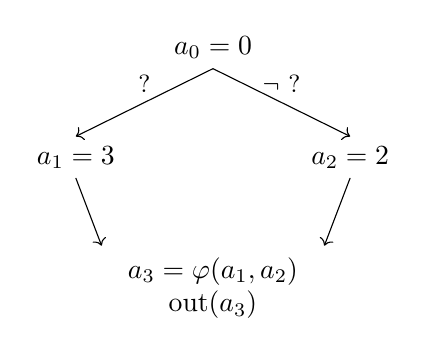
\begin{tikzpicture}[scale=.5]
\node[] (n0) {
  $a_0 = 0$
};
\node[below=of n0] (middle){};
\node[left=of middle] (n1) {
  $a_1 = 3$
};
\node[right=of middle] (n2) {
  $a_2 = 2$
  };
\node[below=of middle] (n3) {
\begin{tabular}{c}
  $a_3 = \phi(a_1, a_2)$ \\
  $\text{out}(a_3)$
\end{tabular}
  };
\draw (n0.south) edge[->] node[above]{\small ?} (n1.north)
      (n0.south) edge[->] node[above]{\small $\neg$ ?} (n2.north)
      (n1.south) edge[->] (n3.north west)
      (n2.south) edge[->] (n3.north east);
\end{tikzpicture}
\end{minipage}
\begin{minipage}[t]{0.30\linewidth}
\null
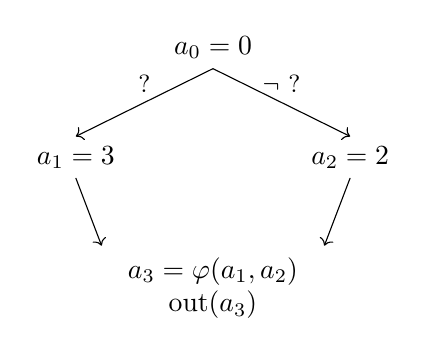
\begin{tikzpicture}[scale=.5]
\node[] (n0) {
  $a_0 = 0$
};
\node[below=of n0] (middle){};
\node[left=of middle] (n1) {
  $a_1 = 3$
};
\node[right=of middle] (n2) {
  $a_2 = 2$
  };
\node[below=of middle] (n3) {
\begin{tabular}{c}
  $a_3 = \phi(a_1, a_2)$ \\
  $\text{out}(a_3)$
\end{tabular}
  };
\draw (n0.south) edge[->] node[above]{\small ?} (n1.north)
      (n0.south) edge[->] node[above]{\small $\neg$ ?} (n2.north)
      (n1.south) edge[->] (n3.north west)
      (n2.south) edge[->] (n3.north east);
\end{tikzpicture}
\end{minipage}


\hfill

A complete treatment of SSA and a profusion of related optimization techniques are available in the excellent SSA Book\cite{ssa-book}. We will still sketch here a few important ideas about SSA, and how they apply more generally. \todo[inline]{This sentence - and the others like it - is unnecessary. It is a given that you should explain just the details that are needed for the report.}

\paragraph{Dominator tree} A central matter in the SSA transform is the question of where in the program $\phi$ nodes insertions are needed. \todo[inline]{By the time I get here I've forgotten what a $\phi$ node is and why they need to be inserted.}
This leads us to introduce the notion of domination: we say that a program point $a$ \emph{dominates} another point $b$ if any path in the CFG \todo{what? spell out the first time} starting at the root node that reaches $b$ has to go through $a$ first. The domination relation is a partial order over program points and is moreover a tree (every initial segment is well ordered). It is usually called the dominator tree. In our case, since every path to a program point has to go through the head of its containing EBB -- and all the points between the head and itself -- we will say that a program point dominates an EBB if it dominates its head. Given an EBB, the program point being its parent in the dominator tree is called the \emph{immediate dominator}.

\todo[inline]{I stopped here.}

The fundamental property of SSA form is then stated as follows: \emph{every use of a variable is dominated by a definition of said variable}. This is considering $\phi$ nodes as being a definition in their EBB but an use at the \emph{predecessor edges origins}. We can deduce a superset of locations where we have to insert $\phi s$ for the property to hold.
We will call the dominance frontier of a program point $a$, noted $\DF(a)$, the set of EBB heads that, while not being dominated by $a$, have predecessors that are. $\DF(a)$ is the set of nodes that one has to visit in order to, starting from $a$, leave its domination.
Following the usual convention, we note $\IDF(a) = \lfp_a\DF$ the iterated dominance frontier of $a$.
If a variable $v$ has two definitions at $a$ and $b$ respectively, we can disambiguate between them by inserting $\phi$ nodes in a subset of $\IDF(a)\cap\IDF(b)$.
This set is an upper bound, because some of those $\phi$ may end up without any use. Computing the minimal $\phi$ placement is harder and requires a form of liveness analysis.
The advantage of the iterated dominance frontier is that $\IDF(a)$ only depends on $a$ and can be cached independently of the variable considered.

In its usual formulation, SSA also implies a renaming of every variable to enforce that, as its name indicates, each one has a single definition site. As a consequence, we can store a global $(\text{name}\to\text{value})$ mapping as a flow-insensitive analysis would, but still get flow-sensitive results.


\paragraph{Our thing?} We take a slightly different approach because we compute the same information as the SSA form but \emph{on the fly}: we assume that use sites of variables cannot be statically determined in advance without computing transfer functions.
It also implies that new use and definition sites can be discovered at an already processed program point in later iterations.
The main reason for this choice is to allow for other quantities than variable values to profit from the sparse infrastructure.
[examples]

Essentially, what we are providing is a generic sparse map implementation from an arbitrary set of names to any value domain.
It can be used to represent any non-relational internal interpreter state of the user's choice.

It is hence inefficient in our case to maintain the renaming property. Instead, when encountering an use, the interpreter walks the dominator tree upward to find the nearest definition.
The SSA property guarantees that this lookup can be done following the tree spine, giving it an $O(\text{dominator tree depth})$ worst case complexity. In practice, the dominator tree is very shallow and wide : in the Julia standard library (around 4MB of sources) the deepest dominator tree is of depth [?].

As for the implementation, we do not materialize $\phi$ instructions: they are kept out of band as a single compound summary information for each EBB head.
They can be efficiently dynamically updated when required by the discovery of new definitions.
We compute the dominator tree and frontiers using the algorithm described in \cite{domtree}.

We have not yet witnessed this process to be a bottleneck. Would it become the case, there are several ideas that could be implemented to lower its cost. The most obvious one being use-forwarding.
As an aside, the choice of EBBs for the program representation offsets the time spent doing this lookup in practice by making common dominator trees shallower.
It is not a worst-case improvement but a welcomed average constant factor gain.

% find somewhere to put this
%Another advantage of EBBs is that the dynamic addition of outbound control flow edges does not require node splitting. It is the case of exception throwing : it would degrade the sparsity of the CFG to conservatively assume that any statement can throw. Our interpreter generates new edges when a transfer function detects a possible raise.

\subsection*{Relational}

As a more general point of view, one can think of $\phi$ nodes as a compact representation of the difference between the interpreter state at an EBB entry and the same state at the dominating exit of its immediate dominator.
It is not readily apparent in the case of a non-relational domain, since this difference is usually represented as an element of the domain itself, i.e., a small name-value mapping that only refers to changed names.

[good example + explanation of a generic translation]
[trash a bit \cite{sparse-nr} for saying relational in their title and only handling packed domains]

\section*{Shape analysis}

[todo some platitudes about shape analysis]

For a moment, we will ignore object fields and summary objects to concentrate on variable aliasing and its sparse structure. We will introduce those back later.
One of the fundamental insight of \cite{ssc} is in the scheme used to describe abstract heap locations.
The abstract address of an object is given by the exact set of stack variables that refers to it.
It means that we can represent the abstract heap as a collection of set of variable names.
The main advantage of this approach compared to the other usual choices, such as allocation site segregation, is that transfer functions operating on objects referenced by variables can \emph{always} perform strong updates.
It is due to the fact that each one of those abstract addresses can refer to at most a single object in any given concrete heap.
Another very important point about this choice is that it provides a canonical way to compare two abstract heaps : there is no ambiguity on the mapping between the nodes, avoiding any kind of graph isomorphism problems.

We refer to \cite{ssc} for the formal deduction rules and computation recipes in this abstract domain.
We will focus here on exposing a way to implement a similar state domain with a sparse representation.
The main inspiration comes from \cite{ssa-alias}: they develop a sparse alias analysis for local variables that we use as a basis for our shape domain. The authors make the following observation.

Assuming that the analyzed code is in SSA form, we can order the set of program variable under the domination relation of their definition.
That being done, it is clear that when transferring the state over a non-dominating edge, we can trim all heap objects of variables whose definition stopped dominating the current control point. In fact, we can always remove any dead variables from our abstract heap, and non-dominating definitions are always dead thanks to the fundamental property of SSA.

To be slightly more precise, here is a sketch of the transfer function for variable assignment and $\phi$ nodes with two predecessors.
\[
\begin{aligned}
&T[x=y](o) = \begin{cases}
o \cup \left\{ x \right\} & \text{if } y \in o \\
o & \text{otherwise}
\end{cases}
\qquad
T[x=y](H) = \Big\{~T[x=y](o)~|~o \in H~\Big\} \\
& T[\tilde{x}=\tilde{y}] = T[x_1=y_1]\circ\dots\circ T[x_n=y_n] \\
&T[\phi(\tilde{x}=\tilde{y},\tilde{z})](H_l,H_r) = \big( T[\tilde{x}=\tilde{y}](H_l)\cup T[\tilde{x}=\tilde{z}](H_r) \big)\cap 2^{\dom(\tilde{x})}
\end{aligned}
\]

where $\text{dom}(\tilde{x})$ is the set of variable having their definition in a dominating position over the $\phi$ node, including itself. It is important to notice that we don't need to remove $x$ from any object when assigning to $x$ since the definition was non-dominating before applying $T$.

As we alluded to in the previous section, one can look at the restriction to dominating definitions as a \emph{summarization} of the state between the $\phi$'s EBB head and its immediate dominator.

From this formulation, we can deduce a sparse format for this simplified ``variable-only'' static shape graph : there is a consequent amount of sharing between subsequent states. In fact, we can see from the transfer functions that they only need to manipulate the ``most recently'' defined variables in each object.
In \cite{ssa-alias}, this sharing is exploited by representing heap objects as sorted singly-linked list with hash-consing. The elimination of redundancy is thus implicitly handled by the data structure.

It has the benefit of keeping the implementation close to the mathematical structure, but forces the algorithm to keep the linked list heads of \emph{all} live heap objects at all control points, defeating some of the sparsity.
We take an alternate route of representing the tree explicitly with pointers in both directions. At the cost of additional lookups along its spine -- much like in the SSA case -- we can cut down the storage at each control point to the set of modified objects. Doing this, we also avoid the need for hash-consing.

\paragraph{Alias tree} The encoding of variable aliasing takes the form of a forest of doubly-linked trees.
Each node is labeled by a variable definition and several nodes can have the same label.
This tree respects the dominance ordering of variable definitions.
The information readily available from this structure is, given a variable $x$, the content of every heap object that $x$ refers to \emph{at the point it was defined}. Each path from a $x$-node to a root is such an object. The set of variable referring to that object is simply the set of labels encountered along the path.

More work has to be done to compute the set of objects referring to $x$ at any point in the program using $x$ : it is the trade-off we make to keep the storage per control point down.
Assuming that $x$ is a definition dominating $a$, the set of tree nodes being the heads of objects that $x$ refers to when the interpreter is at $a$ can be characterized. They are the end-points of paths in the alias tree that starts at an $x$-node and end in a dominating position over $a$.

\begin{algorithm}
\footnotesize
\setlength\columnsep{-1pt}
\begin{multicols}{2}
\begin{algorithmic}
\Function{Materialize}{$H$, $a$, $x$}
\State $d =$ \Call{FindDef}{$x$, $H$, $a$}
\State $R = \left\{\text{nodes of }H\text{ labeled by }d\right\}$
\While{$R$ changed}
\For{$o\in R$}
\State $C = \children(o\text{ in }H)\cap\dom(a)$
\If{$C \neq \emptyset$}
\State $R = \left(R-\{o\}\right)\cup C$
\EndIf
\EndFor
\EndWhile
\State \Return $R$
\EndFunction
\State
\Function{Transfer[$x=y$]}{$H$, $a$}
\State $R =$ \Call{Materialize}{$H$, $a$, $y$}
\For{$r\in R$}
\State $H,o =$ \Call{AddNode}{$H$, $\text{def}\left[a:x\right]$}
\State $H =$ \Call{AddEdge}{$H$, $o \to n$}
\EndFor
\State \Return $H$
\EndFunction
\columnbreak
\Function{Restrict}{$H$, $\tilde{y}$, $n$, $a$, $b$}
\State $R = \{ i \to $ \Call{Materialize}{$H$, $a$, $y_i$} $|~i\in\left[1,n\right]\}$
\While{$R$ changed}
\For{$i \in \left[1,n\right]$}
\State $U = R(i) \cap \big(\dom(b)\cup\roots(H)\big)$
\State $V = \{ \parent(d)~|~d\in R(i) - U\}$
\State $R = R/i\mapsto U\cup V$
\EndFor
\EndWhile
\State \Return $R$
\EndFunction
\State
\Function{Transfer[$\phi(\tilde{x}=\tilde{y},\tilde{z})$]}{$H_{\text{idom}}$, $a$, $H_l$, $a_l$, $H_r$, $a_r$, $n$}
\State $H = H_{\text{idom}}$
\State $R_l =$ \Call{Restrict}{$H_l$, $\tilde{y}$, $n$, $a_l$, $\idom(a)$}
\State $R_r =$ \Call{Restrict}{$H_r$, $\tilde{z}$, $n$, $a_r$, $\idom(a)$}
\State $R = \{ i\mapsto R_l(i)\cup R_r(i)~|~i\in\left[1,n\right]\} $
\For{$d \text{ s.t. } *\mapsto D \in R \text{ and } d\in D$}
\State $V = \left\{i\in\left[1,n\right]~|~d\in R(i)\right\}$
\State $H,n =$ \Call{AddNode}{$H$, $\phi\left[a:\tilde{x}_V\right]$}
\If{$d \in \dom(\idom(a))$}
\State $H =$ \Call{AddEdge}{$H$, $d\to n$}
\EndIf
\EndFor
\State \Return $H$
\EndFunction
\end{algorithmic}
\end{multicols}
\caption*{High level description of transfer for sparse variable alias analysis}
\end{algorithm}

\section*{I can see the future}

[summary of contributions] [technical/impl things] [backward analysis?]

\paragraph{Generic sparsification} We hypothesize that a general transform from dense to sparse state structure underlies the particular one presented in this report and included in our implementation.
Although we do not hope for a fully mechanized way to do such a conversion, it is likely that we could provide a set of generic reusable component to make the implementation as well as the soundness proof of those state domains easier.
As more use cases appear we will try to develop a general framework, both theoretical and implementation-wise, for this process.

\paragraph{User provided optimizations} We briefly hinted at domain-specific optimizations in the introduction.
Our long term plan is to provide hooks in the compiler and the analyzer to allow for user defined analysis and optimization.
Moreover, those should be able to easily build upon the existing infrastructure.
Although the abstract interpreter model is a good fit in that regard, we have not yet found a fully satisfactory equivalent for the optimization side.

As a good example of the envisioned usefulness of this kind of modularity, consider the development of a high-level interface to a BLAS library.
This was not chosen at random since the linear algebra routines are in fact a sizable chunk of the Julia standard library, and BLAS is used as their back end in the common case floating point numeric types.

It is easy to use under a simple model where the output of the computation is freshly allocated memory containing the result. This avoids aliasing bugs, however it is inefficient because it does not take advantage of the specialized BLAS functions that can output the result in place. Reasoning that the two are equivalent if one of the argument (and all its aliases) are dead after the BLAS call is almost impossible to the compiler because it requires understanding of the routine, of which the core is often hand written assembly.
However, the rules of BLAS aliasing are very regular at a high level and someone writing a wrapper for the library could easily, given the right interface, integrate those rules directly as a compiler extension.

As we work towards making the interpreter more accessible, the need for good tooling becomes unavoidable.

\paragraph{Abstract debugging} We would like to provide a common infrastructure aimed at debugging abstract domains.
In its simplest form, this system would open the possibility for a domain to provide small run-time guards checking that the state conforms to what was inferred.
The analyzer would then, in ``verification'' mode, insert those guards in the code before running it, along with the necessary information to trace back the exact transfer function that computed an unsound result.
This would obviously not replace a formal proof of soundness but would help weed out implementation errors by large scale testing on the consequent amount of freely available Julia source.

\paragraph{Visualization} As a way to help implementation work, a graphical visualization of the interpreter was hastily put together.
The usefulness of this tool exceeded our -- admittedly low -- expectations. [maybe screenshot in annex]
We believe that interactive feedback is a key aspect of allowing users with no particular background in program analysis to develop an understanding of the -- in fact quite natural -- underlying model.

\newpage

\begin{thebibliography}{9}
\bibitem[BEK14]{julia-paper} Jeff Bezanson, Alan Edelman, Stefan Karpinski, Viral B. Shah -- \emph{Julia: A fresh approach to numerical computing} (2014) \verb~arXiv:1411.1607~
\bibitem[SMRW98]{ssc} Sagiv, Mooly, Thomas Reps, Reinhard Wilhelm -- \emph{Solving shape-analysis problems in languages with destructive updating} (TOPLAS 1998)
\bibitem[CC77]{absint-cousot} Patrick Cousot, Radhia Cousot -- \emph{Abstract interpretation: a unified lattice model for static analysis of programs by construction or approximation of fixpoints} (SIGPLAN 1977)
\bibitem[Bez15]{jeff-phd} Jeff Bezanson -- \emph{Abstraction in Technical Computing} (2015)
\bibitem[LoA15]{ssa-book} ``Lots of authors'' -- \emph{Static Single Assignment Book} (2015)
\bibitem[NL09]{ssa-alias} N. A. Naeem, O. Lhotak -- \emph{Efficient alias set analysis using SSA form} (ISMM 2009)
\bibitem[OHLLY12]{sparse-nr} Hakjoo Oh, Kihong Heo, Wonchan Lee, Woosuk Lee, Kwangkeun Yi -- \emph{Design and Implementation of Sparse Global Analyses for C-like Languages} (PLDI 2012)
\bibitem[CDHK01]{domtree} Cooper, Keith D., Timothy J. Harvey, Ken Kennedy -- \emph{A simple, fast dominance algorithm} (2001)
\bibitem{julia-web} \verb~http://julialang.org~
\bibitem{gf-web} \verb~https://github.com/carnaval/green-fairy~
\end{thebibliography}

\end{document}
